\documentclass[dvipdfmx]{jarticle}
\usepackage{graphicx}
\usepackage[top=30truemm,bottom=30truemm,left=25truemm,right=25truemm]{geometry}
\usepackage{listings,jvlisting}
\usepackage{url}
\title{計算機援用工学前半レポート}
\author{ソフトウェア科学コース\\09B22084山久保孝亮}
\date{\today}


\lstset{
  basicstyle={\ttfamily},
  identifierstyle={\small},
  commentstyle={\smallitshape},
  keywordstyle={\small\bfseries},
  ndkeywordstyle={\small},
  stringstyle={\small\ttfamily},
  frame={tb},
  breaklines=true,
  columns=[l]{fullflexible},
  numbers=left,
  xrightmargin=0zw,
  xleftmargin=3zw,
  numberstyle={\scriptsize},
  stepnumber=1,
  numbersep=1zw,
  lineskip=-0.5ex
}

\begin{document}
\maketitle
\section{選んだ理由}
今回私が選んだ授業で出てくるワードは暗号化技術である.特に,POODLEによるSSLv3の脆弱性について詳しく調査した.私がこのテーマを選んだ理由としては,この脆弱性が原因でガラケーからスマホへの移行が進んだという講義内の話に関心を持ったためである.
\section{調査の概要}
\subsection{技術の背景}
SSLv3は暗号化通信用のプロトコルであり,ドコモ,au,ソフトバンクなどのキャリアが提供するiモードブラウザ等でサポートされていた.\cite{0}
SSLv3で利用される暗号はCBC方式のブロック暗号を選択することができ,以下の図1のように一定のサイズのブロックごとに暗号化・復号を行う.\cite{1}図1では直前の暗号文と複合処理を行った暗号文をXORしている.
\begin{figure}[h]
    \centering
    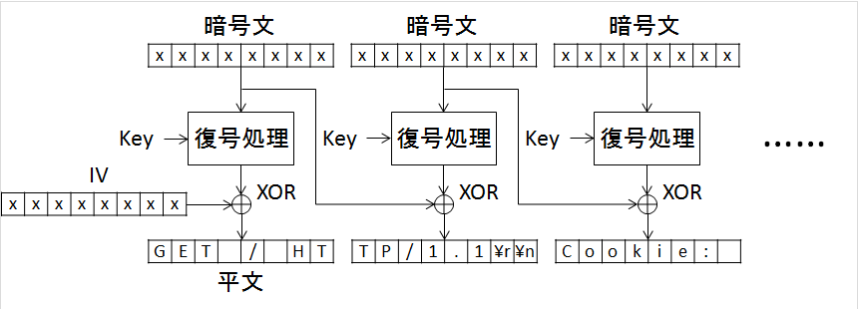
\includegraphics[width = 8cm]{CBC.png}
    \caption{ブロック暗号の復号処理}
\end{figure}
\\このとき,一定サイズごとに復号を行うため,平文の最後がブロック長に比べて中途半端な長さになることが発生してしまう.その場合はダミーの文字を入れて調整を行っており,この文字をPaddingという.また,一番最後のバイトはPadding長として規定されており,例えば平文がブロックサイズちょうどであっても,Padding長を格納するために
ダミー文字とPadding長のみのブロックが追加される.
\subsection{手法}
POODLEでは2.1で述べたPadding長を利用して暗号文から平文を解読する.
\\まず解読したい暗号文のブロックをコピーし,Padding長を格納しているブロックと置き換えてサーバに送信する.
これにより,基本的にはPadding長が変わるためサーバからエラーが返されるが,Padding長は1byteで表されるため$\frac{1}{2^8}=\frac{1}{256}$の確率で一致してしまう.これが偶然一致した場合サーバからはエラーが返されないので
攻撃者はPadding長が一致したことを知ることができる.さらに,図1のようにCBC方式のブロック処理では復号処理を行った暗号文と直前の暗号文をXORするのみであるため,直前の暗号文を攻撃者が意図した内容に変更することでエラーが返されない場合のPadding長を求めることができる.\cite{2}
\\
その後,以下の図2のようにすることでコピーした暗号文の復号結果の最下位バイトを知ることができる.\cite{1}
\begin{figure}[h]
  \centering
  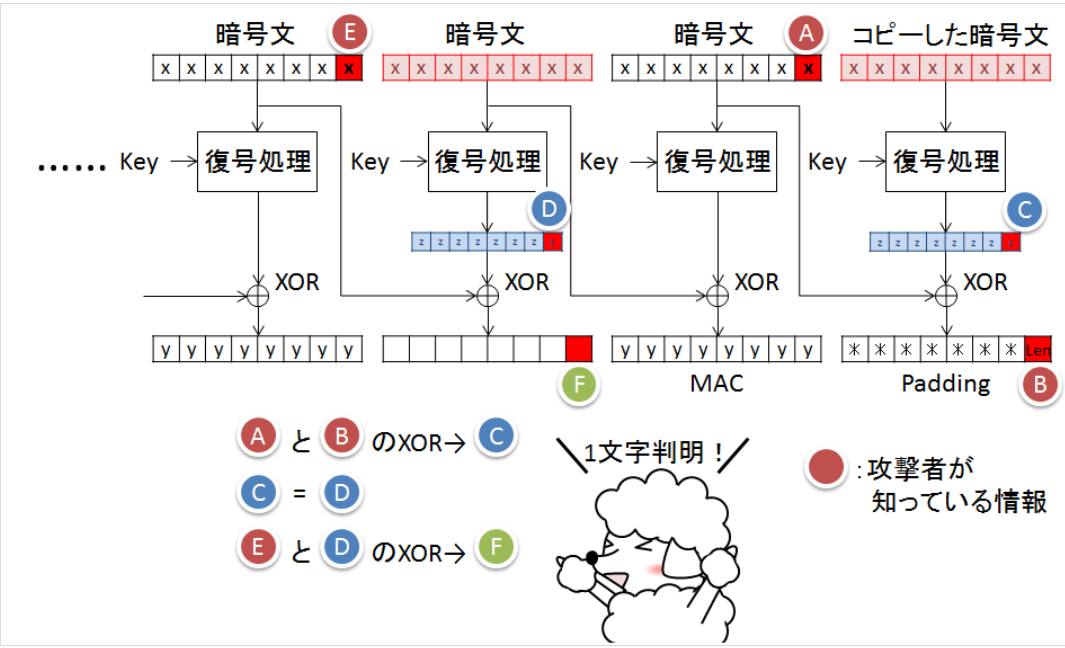
\includegraphics[width = 8cm]{POODLE.png}
  \caption{ブロック暗号の復号処理}
\end{figure}
\\右下のBの赤い部分は上で求めたPadding長であり,Aは攻撃者が変更した暗号文である.右二列はコピーした暗号文に対して復号処理が行われCが生まれ,これとAをXORすることでBになることを表している.左から二番目は解読したい暗号文が本来あった位置を表し,これに対し復号処理が行われDが生まれている.
このとき,CとDはどちらも同じ暗号文に対して復号処理を行った結果でありその値は同じになるはずである.また,Eの暗号文の最下位バイトを攻撃者は確認できるため解読したい暗号文の最下位バイトをXORすることで求められる.
\subsection{結果}
HTTPのプロトコルを使用すれば求めたい平文のbyteの位置を変更することができるため,2.2の処理を繰り返し行うと暗号文を解読することができる.
\section{自分の見解}
今回私がPOODLEの脆弱性について詳細に調査して,一見解読不可能に見えるような仕組みのセキュリティでも解読する方法が存在するということについてとても驚いた.
そして,現在普及しているプロトコルにおいても今後脆弱性が発見される可能性があるということを再認識させられた.ただ,脆弱性があるという事のみを知るのではなく,どのような脆弱性があるのか,何が原因だったのかを把握することは
情報セキュリティの分野だけでなく全ての分野において持つべき姿勢であると考えた.常に理解する姿勢を崩さないことは来年以降の研究に役立つと思って継続していきたいと思う.
\begin{thebibliography}{99}
    \bibitem{0} \url{https://qiita.com/harukasan/items/dee779c0a3f624758230} 12/16アクセス
    \bibitem{1} \url{https://engineering.dena.com/blog/2014/10/poodle/} 12/16アクセス
    \bibitem{2} \url{https://partender810.hatenablog.com/entry/2021/06/08/225105} 12/18アクセス
\end{thebibliography}
\end{document}